%%%%%%%%%%%%%%%%%%%%%%%%%%%%%%%%%%%%%%%%%%%%%%%%%%%%%%
%
% This file defines the style for your report
% You don't need to edit it any more, if not to change the authors name.
%
% Search below for the keyword:   GROUP
% insert your group number
%
% Search below for the keyword:   AUTHORS
% insert the name of the authors
%
% If you want to compile your document you have TWO ways
% depending on the fact that 
% 	1) you have inserted only postscript images in your .tex file 
%		---> then go to MODE 1
%	2) you have inserted other kind of images (jpg, pdf, ...) in your .tex file
%		---> then go to MODE 2
%
% MODE 1 
% Type:
% 	latex homebook.tex
%
% If the compilation runs successfully and you want to see the results type:
% 	xdvi homebook.dvi &
% and use the menus to go through the document
%
% If you want to create a pdf type:
% 	dvipdfm homebook.dvi
%
% a homebook.pdf file is created
% you can see it using the command:
% 	acroread homebook.pdf &
%
%
% MODE 2
% Type:
%	pdflatex homebook.tex
%
% If the compilation runs successfully you directly have the pdf file
% and you can see it using the command:
%       acroread homebook.pdf &
%
% 
%%%%%%%%%%%%%%%%%%%%%%%%%%%%%%%%%%%%%%%%%%%%%%%%%%%%%%

\documentclass[10pt,  english, makeidx, a4paper, titlepage, oneside]{book}
\usepackage{babel}
\usepackage{fancyhdr}
\usepackage{makeidx}
\usepackage{titlesec}
\usepackage{listings}
\usepackage{booktabs}

\newenvironment{listato}{\footnotesize}{\normalsize }

%\pagestyle{empty}

\textwidth 15.5cm
\textheight 23cm
\topmargin -1cm
\oddsidemargin -0.5cm
\linespread{1.1}

\pagestyle{fancy}
\lhead{}
\chead{System design project} %MODIFICARE IL NOME
\rhead{}
\lfoot{}
\cfoot{}
\rfoot{}
\rhead{\thepage}

\usepackage{graphicx}
\usepackage{amsmath}
\usepackage{amsfonts}
\usepackage{amsthm}
\usepackage{amssymb}
%\oddsidemargin -1.1cm
\usepackage{graphicx}
\usepackage{caption}
\usepackage{float}
\usepackage{amsmath}
\usepackage{amssymb}
\usepackage{amsfonts}
\usepackage{amsthm}
\usepackage{subscript}
\usepackage{empheq}
\usepackage{verbatim}
\usepackage{fancyvrb}
\usepackage{datetime}
\usepackage{hyperref}


\lstdefinelanguage{VHDL}{morekeywords={library,use,all,entity,generic, is,port,in,out,end,architecture,of,begin,and,if,then,else,elsif,process},morecomment=[l]--}

\lstdefinestyle{vhdl}{language = VHDL, basicstyle = \ttfamily, keywordstyle = \color{keyword}\bfseries, commentstyle = \color{comment}}

\titleformat{\chapter}[display]
{\normalfont\Large\filcenter\sffamily}
{\titlerule[0.5pt]%
\vspace{1pt}
\titlerule
\vspace{1pc}
\LARGE\MakeUppercase{\chaptertitlename} \thechapter
}
{1pc}
{\titlerule
\vspace{1pc}
\Huge}
{
	\rfoot{\textcopyright Garolla, Jiang, Forno, Buttafuoco, Bellino\\
		Project 8 - IP-core Manager for FPGA-based Designs (RT level)}
	}

\makeindex

\begin{document}

\frontmatter
\begin{titlepage}
\vspace{0cm}
\centerline{

\includegraphics[width=3cm]{./logopoli}} 
\vspace{0.5cm}
\centerline{\LARGE Politecnico di Torino}
\vspace{2cm}
\centerline{\Huge\sf System design project}
\vspace{1.5cm}
\centerline{\huge \sf Project8 }
\bigskip
\centerline{\huge\sf IP-core Manager for FPGA-based Designs (RT level)}
\vspace{1.2cm}
\centerline{\huge\sf Report of the Milestones}
\vspace{1.5cm}
%\centerline{\Large Master degree in Computer Engineering}
%\centerline{\Large Specialization in Embedded Systems}
\bigskip
\vspace{0.5cm}
%%%%%%%%%%%%%%%%%%%%%%%%%%%%%%%%%%%%%%%%%%%%%%%%%%%%%%
%
\centerline{\large Referents: }
\centerline{\large Prof. Paolo Ernesto Prinetto}
\centerline{\large PhD. Student Giuseppe Air\`{o} Farulla}
\bigskip
\vspace{1cm}
%
%%%%%%%%%%%%%%%%%%%%%%%%%%%%%%%%%%%%%%%%%%%%%%%%%%%%%%
% GROUP
% Change the name of your group below
%
\centerline{\large Authors:}
\bigskip
%
%%%%%%%%%%%%%%%%%%%%%%%%%%%%%%%%%%%%%%%%%%%%%%%%%%%%%%
% AUTHORS
% Change the name of the Group participants here
%
\centerline{\large Emanuele Garolla}
\centerline{\large Gina Jiang}
\centerline{\large Evelina Forno}
\centerline{\large Francesco Buttafuoco}
\centerline{\large Salvatore Bellino}
%
%%%%%%%%%%%%%%%%%%%%%%%%%%%%%%%%%%%%%%%%%%%%%%%%%%%%%%
\vspace{2cm}
\newdateformat{monthyeardate}{%
	\monthname[\THEMONTH], \THEYEAR}
\centerline{\large \monthyeardate\today}
\end{titlepage}
 %\include{content/frontmatter/acknowledgements}
 
\newenvironment{acknowledgements}%
{\cleardoublepage\thispagestyle{empty}\null\vfill\begin{center}%
		\bfseries\textbf{ \huge Acknowledgements}\end{center}}%
{\vfill\null}



%\tableofcontents

\mainmatter
%%%%%%%%%%%%%%%%%%%%%%%%%%%%%%%%%%%%%%%%%%%%%%%%%%%%%%
%    
% HERE IS WHERE YOU INCLUDE YOUR CHAPTERS
%
%%%%%%%%%%%%%%%%%%%%%%%%%%%%%%%%%%%%%%%%%%%%%%%%%%%%%
% This will help you in writing your homebook
% Remember that the character % is a comment in latex
%
% chapter 1
\chapter{Protocol}
\label{chap1}

%%%%%%%%%%%%%%%%%%%%%%%%%%%%%%%%%%%%%%%%%%%%%%%%%%%%%%%%%%%
% you can organize a chapter using sections -> \section{Simulating an inverter}
% or subsections -> \subsection{simulating a particular type of inverter}

%%%%%%   First section

\section{Read Transaction}

Whenever the CPU wants to begin a transaction with one of the IPs present on the FPGA, it writes at address 0 of the buffer a data packet compliant with the following specifications: 
\bigskip
\begin{center}
	\begin{tabular}{ | l | l |  l | l | l |}
		
		15 & 14 & 13 & 12 & 11 \qquad \qquad 0 \\ \hline
		R/W & INT & B/E & UNUSED & IP ADDR\\ \hline
		
		
		\hline
	\end{tabular}
\end{center}

\bigskip
\begin{center}
	\begin{tabular}{ | c | p{7 cm} |  l |}
		\hline
		Bit(s) & Purpose & Value(s)  \\ \hline
		Bit 15 & It specifies whether the transaction is a read or write transaction.  & Read = 0, Write = 1 
		 \\ \hline

		Bit 14 & Specifies whether the current transaction is due to an interrupt request   & Normal = 0, Interrupt  =  1
		\\ \hline
		
		Bit 13 & Signals the begin/end of a transaction & Begin  = 1, End = 0 
			\\ \hline
		Bit 12 & Unused & Unused 	
			
				\\ \hline		
				Bit 11-0 & The physical address of the target IP (in general is different form the IP number) &
				From 0 up to N-1  \\
		 
		
		
		\hline
	\end{tabular}
\end{center}
\bigskip
The various step for a read operations are:\\
\begin{enumerate}
	\item \textbf{Control word for the IP manager}\\
	 The CPU writes at address 0 the control word for the IP manager.
	 For example it could write
	 
	 \begin{center}
	 	\begin{tabular}{ | l | l |  l | l | l |}
	 		
	 		15 & 14 & 13 & 12 & 11 \qquad \qquad 0 \\ \hline
	 		R/W & INT & B/E & UNUSED & IP ADDR\\ \hline
				0 & 0 & 1 & * & 000000000000\\ \hline	 		
	 		
	 		\hline
	 	\end{tabular}
	 \end{center}
	
	 \bigskip
	 Then the buffer will give this data to the IP CORE manager (\textit{row\_0})
	 
	 \item \textbf{IP manager will activate the transaction}\\
	 The IP manager will enable the selected IP Core and give the right input to the switch.
	 
	 \item \textbf{IP core gives the data}\\
	 The selected IP core will write some data to the buffer, thus the CPU can now read the value of the IP CORE from the buffer.
	 
	 \item \textbf{Close transaction}\\
	 The CPU writes at address 0 the control word for the IP manager to close the transaction.
	 In this case it will disable all the IP Cores.
	 
	 \begin{center}
	 	\begin{tabular}{ | l | l |  l | l | l |}
	 		
	 		15 & 14 & 13 & 12 & 11 \qquad \qquad 0 \\ \hline
	 		R/W & INT & B/E & UNUSED & IP ADDR\\ \hline
	 		0 & 0 & 0 & * & 000000000000\\ \hline	 		
	 		
	 		\hline
	 	\end{tabular}
	 \end{center}
	 
\end{enumerate}
% Below is shown how you can insert a figure. If you give a label to the figure, you can refer to the figure using \ref{figure_label} as shown above. 
\bigskip
\bigskip

 \begin{figure}[h]
 	\centering
 	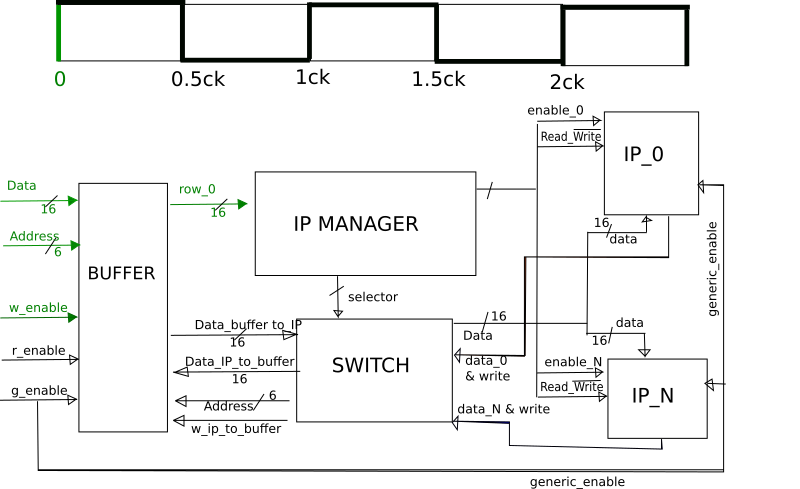
\includegraphics[scale=0.75]{chapters/figures/read_0.png}  
 	\caption{\textbf{Write the control signal on address 0 of the buffer.} \\Since the buffer is asynchronous, it will give this info to the IP Manager as soon as possible with the signal \textit{row\_0}}
 	\label{fig:0}
 \end{figure}
 
  \begin{figure}[h]
  	\centering
  	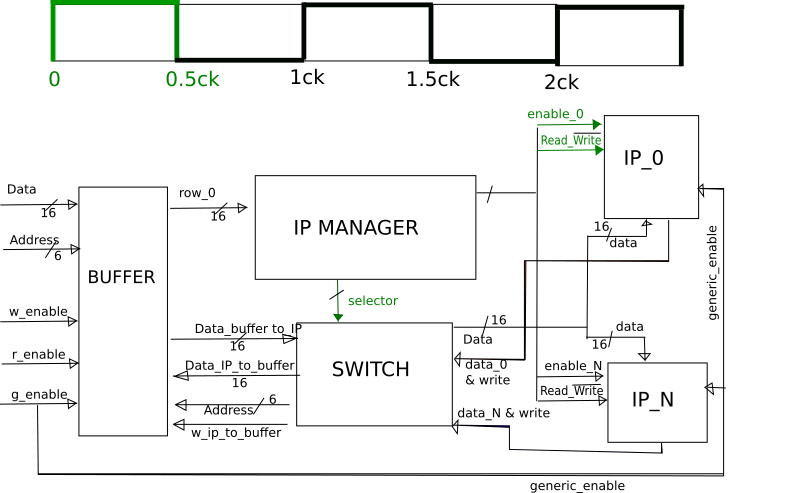
\includegraphics[scale=0.75]{chapters/figures/read_1.png}  
  	\caption{\textbf{IP Manager activate the transaction}. \\The IP Manager will enable the selected IP on the falling edge of the clock. The selected IP will do nothing because it is positive edge sensitive. In the meantime the IP Manager will give the right value to the switch. Even if the switch is active, both the buffer and the IP\_0 are uneffected: \textit{w\_ip\_to\_buffer} and\textit{ Write} to the IP signals are '0'}
  	\label{fig:1}
  \end{figure}
  
   \begin{figure}[h]
   	\centering
   	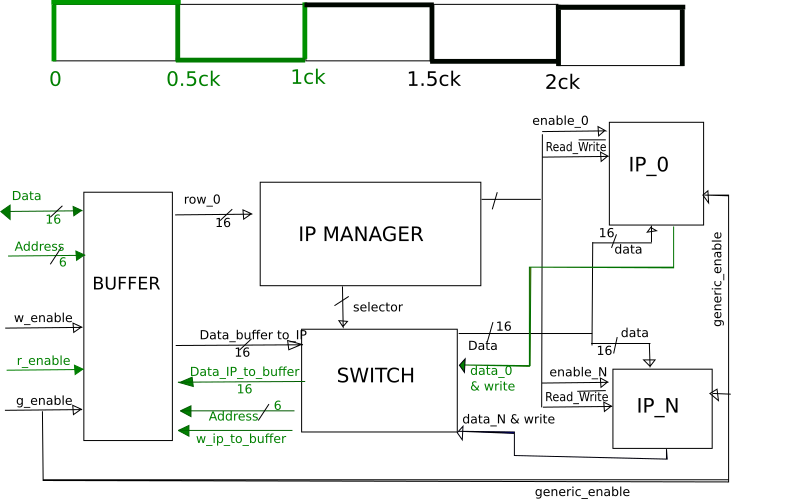
\includegraphics[scale=0.75]{chapters/figures/read_2.png}  
   	\caption{\textbf{IP core gives the data.} \\
   		Now that we have the rising edge of the clock, the IP core is active, and will give the data to the switch which will forward it to the buffer. Both the switch and the Buffer are always active (asynchronous). That means that the CPU can ask the buffer to read the new value.\\\\
   		If there were any problems (e.g. latency), the CPU can ask the buffer to read in this clock cycle and check tha value on the \textit{Data} signal on the next clock cycle.}
   	\label{fig:2}
   \end{figure}
   
    \begin{figure}[h]
    	\centering
    	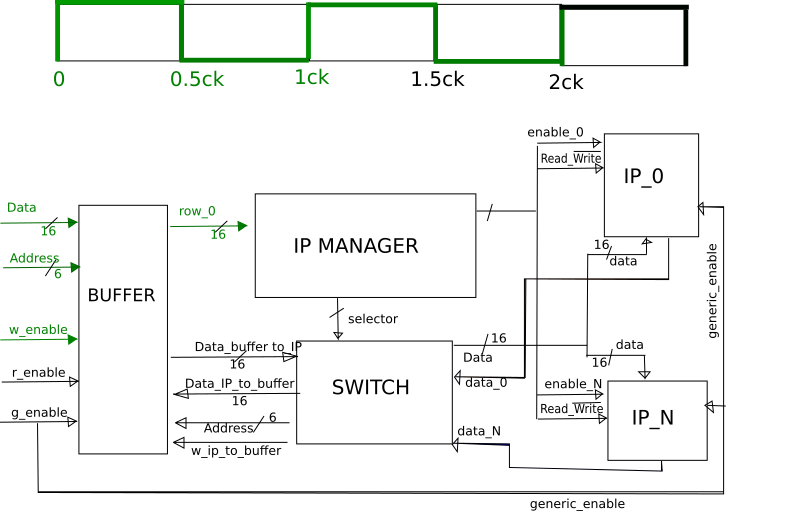
\includegraphics[scale=0.75]{chapters/figures/read_3.png}  
    	\caption{\textbf{Close transaction}\\ The CPU has to tell to the IP Manager to disable all the IP Core \textit{row\_0}}
    	\label{fig:3}
    \end{figure}
    
     \begin{figure}[h]
     	\centering
     	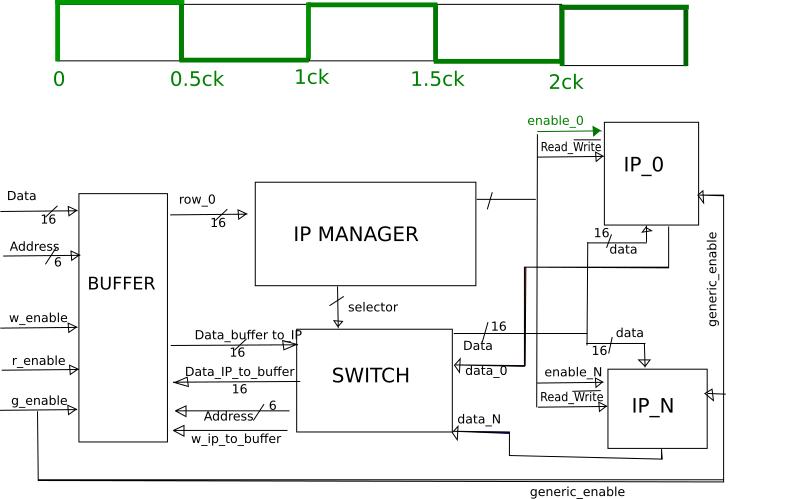
\includegraphics[scale=0.75]{chapters/figures/read_4.png}  
     	\caption{\textbf{Transaction closed}\\ IP manager disables the IP core}
     	\label{fig:4}
     \end{figure}

%%%%%%%%%%%%%%%%%%%%%%%%%%%%%%%%%%%%%%%%%%%%%%%%%%%%
% This will help you in writing your homebook
% Remember that the character % is a comment in latex
%
% chapter 1

%%%%%%%%%%%%%%%%%%%%%%%%%%%%%%%%%%%%%%%%%%%%%%%%%%%%%%%%%%%
% you can organize a chapter using sections -> \section{Simulating an inverter}
% or subsections -> \subsection{simulating a particular type of inverter}

%%%%%%   First section

\chapter{Report on the activities held}
\begin{table}[h]
	\begin{tabular}{p{2.1cm}|  p{13.5cm}}
\multicolumn{2}{p{15.0cm}}{ \LARGE{{Setting up the group and the environment to work in team}}}\\
\hline \hline 
\multicolumn{2}{p{1.0cm}}{ \Large{{}}}\\
	07/03/2017 & \textbf{Group formation and selecting the homework}\\
	12/03/2017& Discussing the possibility to work in a team of 4 people, and the preference of the homework available. \\
	\multicolumn{2}{p{1.0cm}}{ \Large{{ }}}\\	
	15/03/2017 & \textbf{Confirmation of the group}	 \\
	&It has been announced the groups and the related project. Another member joined the team. \\
	&We also exchanged the email address and the telephone number to fasten the communication between members abroad (Whatsapp, Skype, Telegram...).\\
		\multicolumn{2}{p{1.0cm}}{ \Large{{ }}}\\
		22/03/2017 & \textbf{Redmine platform}\\
		27/03/2017& Set-up the Redmine platform. Understanding how to use it, register, open a new topic, upload file, register time. \\
		\multicolumn{2}{p{1.0cm}}{ \Large{{ }}}\\	

\end{tabular}
\end{table}	
\begin{table}[h]
	\begin{tabular}{p{1.9cm}|  p{13.5cm}}	
	\multicolumn{2}{p{15.0cm}}{ \LARGE{{Understanding the environment and the requirements}}}\\
	\hline \hline 
	\multicolumn{2}{p{1.0cm}}{ \Large{{}}}\\
	22/03/2017 & \textbf{SEcube documentation}\\
	03/04/2017& Reading the SEcube documentation and write down the analysis.\\
	\multicolumn{2}{p{1.0cm}}{ \Large{{ }}}\\		
	03/04/2017 & \textbf{Communication Protocol v.1.0}\\
	10/04/2017& Meeting with the professor on $ 3^{rd} $ April and on $ 4^{th} $ April. Then we discussed with other projects team (project 13, 7, 14) to enhance the protocol.
	\\ \multicolumn{2}{p{1.0cm}}{ \Large{{ }}}\\	
		11/04/2017 & \textbf{Communication Protocol v.2.0}\\
		20/04/2017 & During Easter Holyday, the project 13 sent the second version to the teacher, but other modifications were needed.\\
		\multicolumn{2}{p{1.0cm}}{ \Large{{ }}}\\	
		26/04/2017 & \textbf{Communication Protocol v.3.0}\\
		02/05/2017 & Discussion with the team involved. Then the project 13 submitted the final protocol.
\end{tabular}
\end{table}	
\begin{table}
	\begin{tabular}{p{2.1cm}|  p{13.5cm}}
		\multicolumn{2}{p{15.0cm}}{ \LARGE{{Project Development and Documentation}}}\\
		\hline \hline 
		\multicolumn{2}{p{1.0cm}}{ \Large{{}}}\\
		18/04/2017 & \textbf{GIT setup and backbone in VHDL}\\
		23/04/2017& Read GIT manual, GIT set up.\\
		 &Write in VHDL the interface of all the components.\\
		\multicolumn{2}{p{1.0cm}}{ \Large{{ }}}\\	
		21/04/2017 & \textbf{Presentation of the $ 26^{th} $ April}	 \\
		26/04/2017 & It has been requested 3 slides talking about:\\
		& \quad- Gantt\\
			&\quad- Milestones - Deliverables\\
			&\quad- Issues already closed - still open..\\

	\multicolumn{2}{p{1.0cm}}{ \Large{{}}}\\
		02/05/2017 & \textbf{Developemnt of the IP-core Manager and documentation}\\
		10/06/2017&-Split the work among us\\
			& - Deciding the communication among the components\\
			& - Write down the architecture, upload it on GIT, perform some tests\\
			& - Report timing and area and synthesys results with LATTICE Diamond\\
			& - Documentation and presentation\\
	%	10/06/2017& We discussed how to split the work among us, if there were any problem between the communication between some components.\\
	%	&We then wrote the architecure in VHDL, upload it on GIT, do some test, write some documentations and presentation.\\
	%	&Finally we tried to some synthesys on the LATTICE Diamond software and tried to the source file on the board.\\
		\multicolumn{2}{p{1.0cm}}{ \Large{{ }}}\\	
		
	\end{tabular}
\end{table}

\begin{figure}[h!]
	\centering	
	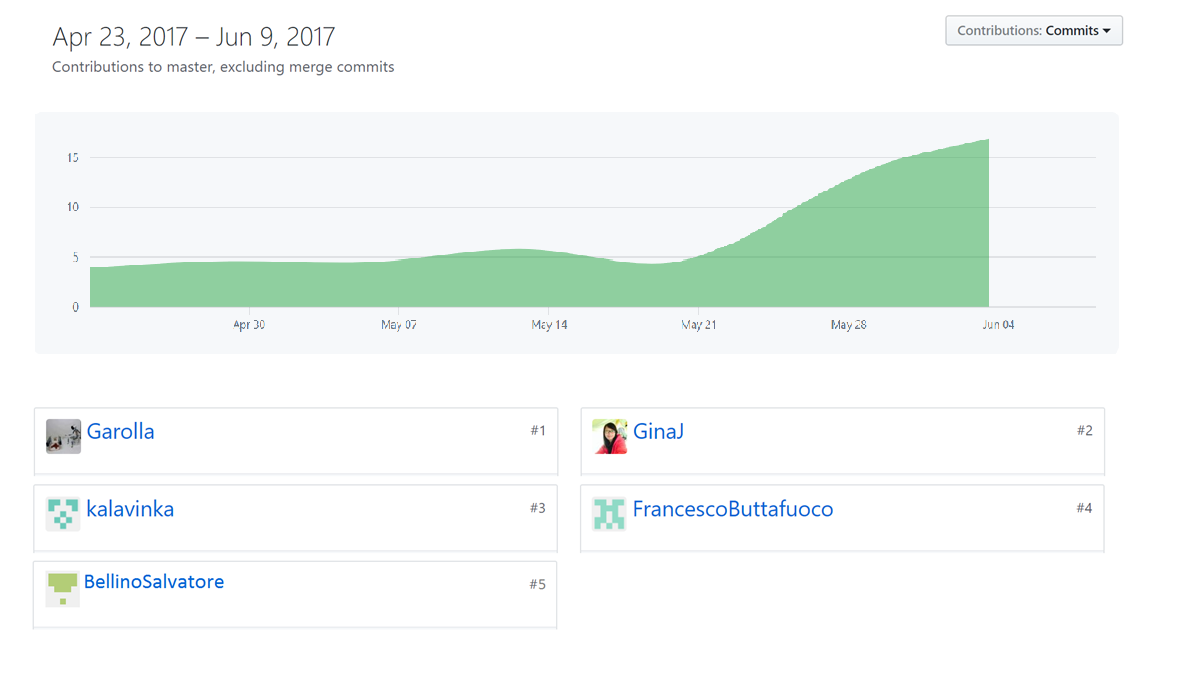
\includegraphics[width=\textwidth]{chapters/git.png}  
	\caption{Our project on GIT, with us as contributors} 
	\label{git}
\end{figure}	
\begin{table}
	\begin{tabular}{p{3.5cm}|  p{12.1cm}}
		\multicolumn{2}{p{15.0cm}}{ \LARGE{{Assignment of the tasks }}}\\
		\hline \hline 
		\multicolumn{2}{p{1.0cm}}{ \Large{{}}}\\
		GAROLLA Emanuele& -Backbone of project in VHDL\\
		& -Dual port buffer 64x16 (Behavioral)\\
		&-Assemble all files\\	
	 &-Final Testbench of the overall architecture	 \\
		 & -Slides\\
		
		\multicolumn{2}{p{1.0cm}}{ \Large{{}}}\\
		JIANG Gina& -Documentation for the $ 26^{th} $ April\\
		&-Documentation for the $ 27^{th} $ May\\
		&-Report timing and area, synthesys result (LATTICE Diamond)\\
		&-Technical report\\
		\multicolumn{2}{p{1.0cm}}{ \Large{{ }}}\\
		
		BELLINO Salvatore& -Dual port buffer 64x16 (Behavioral)\\
		&\qquad -Register 0\\
		&\qquad -Register 16 bits\\
		&\qquad -Decoder\\
		&-Testbench for the data buffer\\
		&-Slides	\\
			
%			\end{tabular}
%		\end{table}	
%		\begin{table}
%			\begin{tabular}{p{3.5cm}|  p{12.1cm}}
%					\multicolumn{2}{p{15.0cm}}{ \%LARGE{{Assignment of the tasks (part 2/2)}}}\\
%					\hline \hline
\multicolumn{2}{p{1.0cm}}{ \Large{{ }}}\\	
		FORNO Evelina& -Dummy IP-core\\
		&-Adder IP-core (FSM with 3 stage)\\
		&-First version of testbench\\
		&-Slides\\
		\multicolumn{2}{p{1.0cm}}{ \Large{{ }}}\\
		BUTTAFUOCO & -IP-Manager Behavioral\\
		Francesco&\qquad-Enabling the right IP core\\
		&\qquad-Propagate the right Data from the selected IP core to the Buffer/CPU\\
		&\qquad-Interrupt Handler\\
		&-Slides\\	
	\end{tabular}
\end{table}
\begin{figure}[h!]
	\centering	
	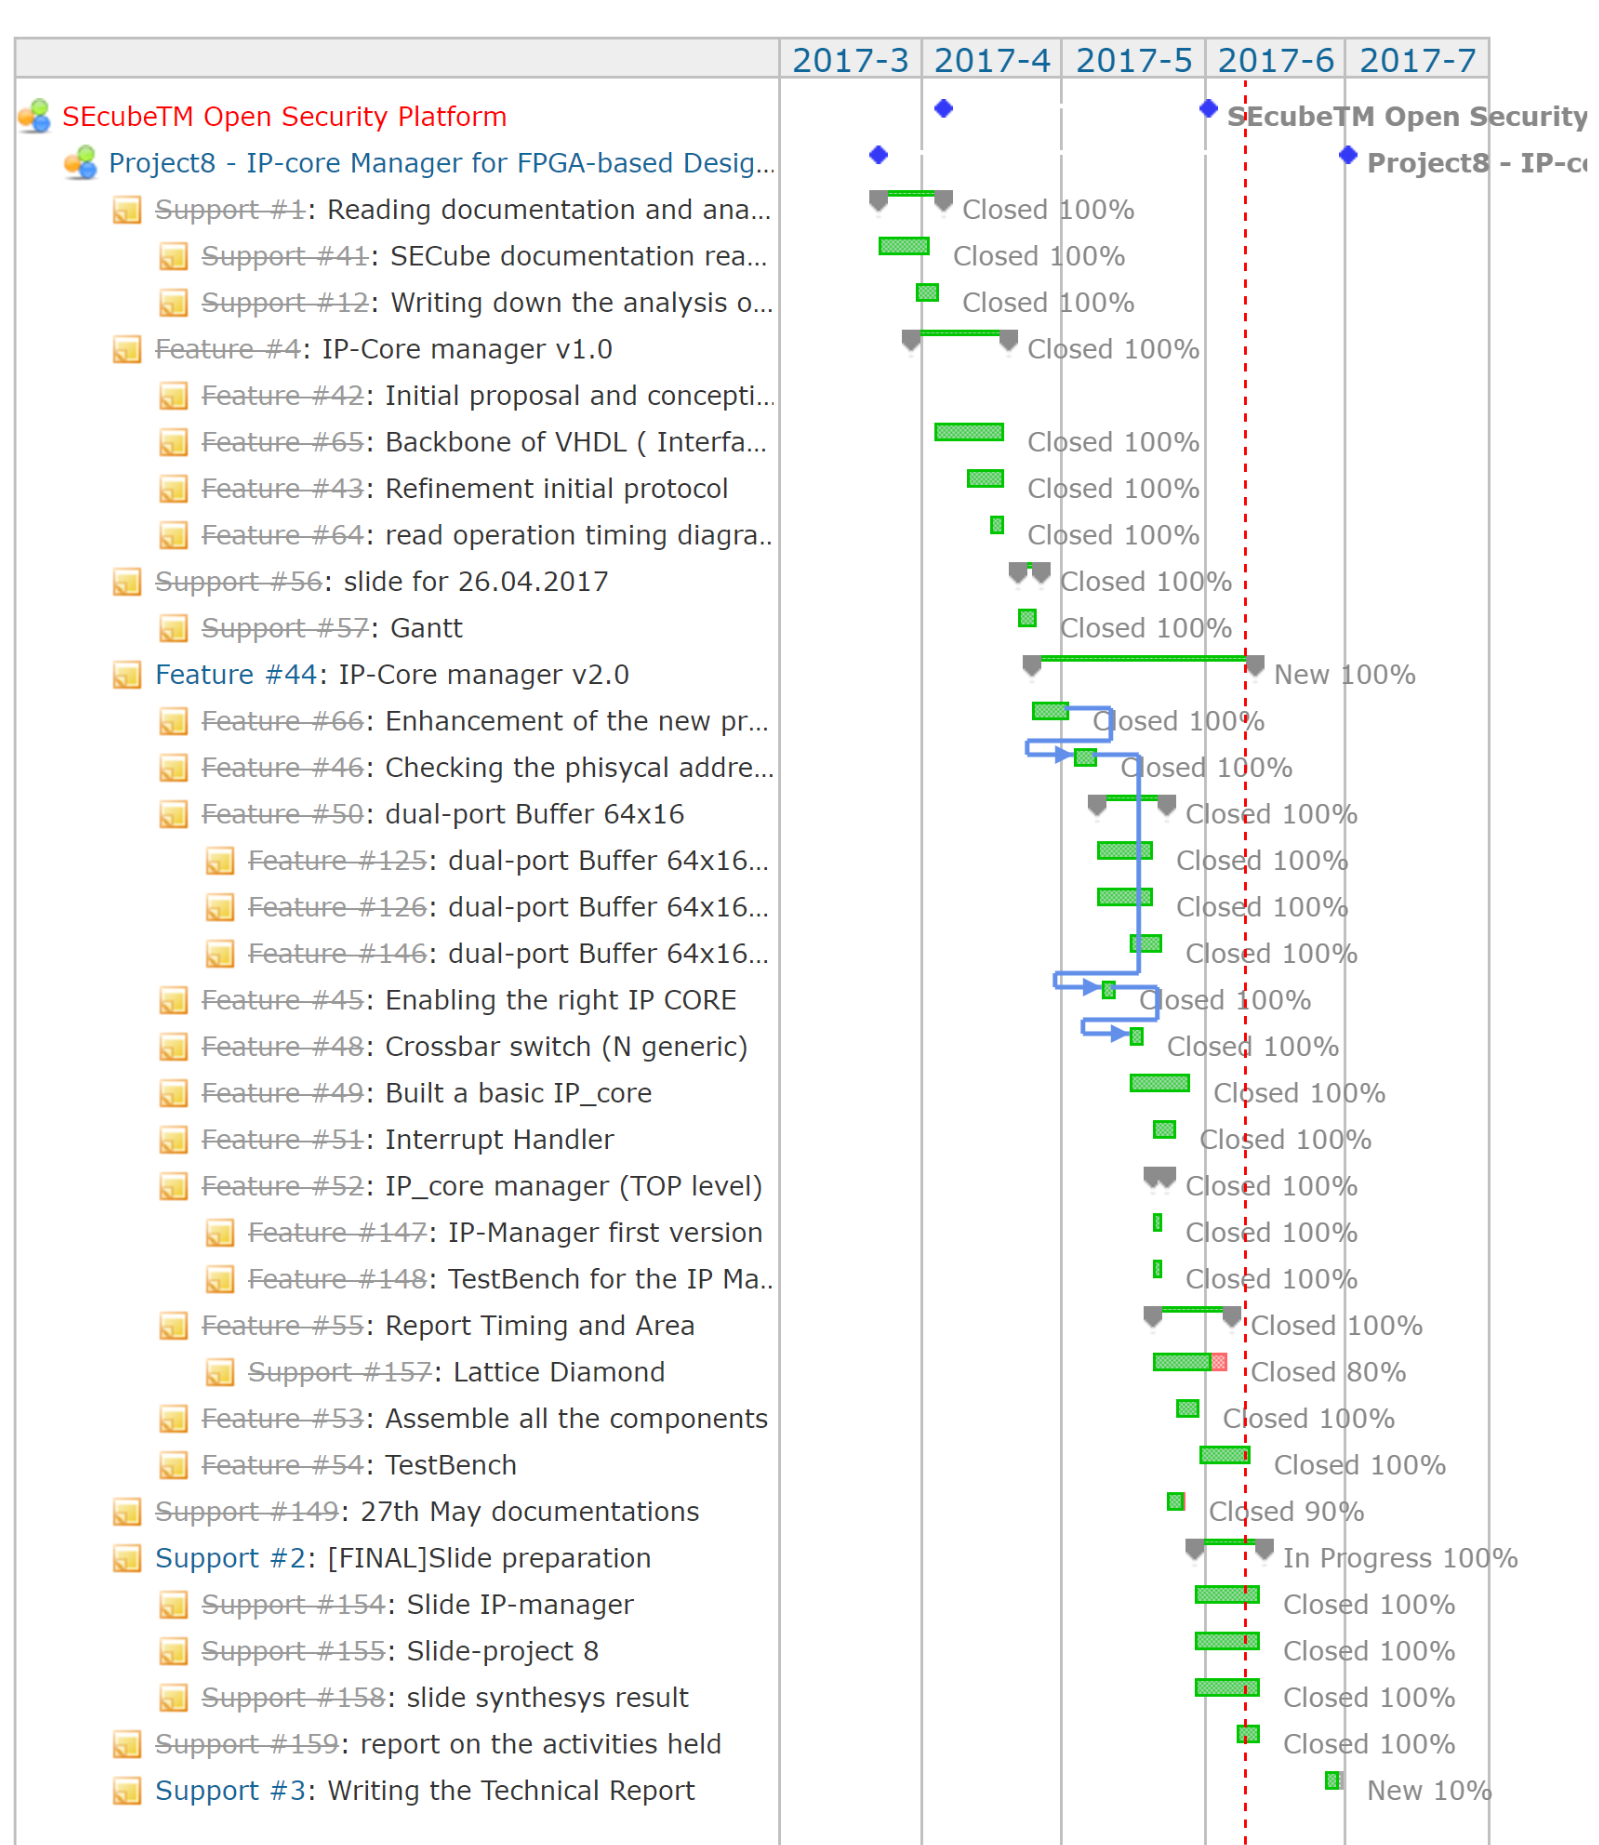
\includegraphics[height=0.65 \textheight]{chapters/gantt.png}  
	\caption{Gantt chart of our project} 
	\label{gantt}
\end{figure}	
% \input{./chapters/chap_name}
% and so on
%
%%%%%%%%%%%%%%%%%%%%%%%%%%%%%%%%%%%%%%%%%%%%%%%%%%%%%%
%    
% HERE IS WHERE YOU INCLUDE YOUR APPENDICES (IF ANY)
%
%\appendix
%%%% Appendix A
\chapter{Adder behavioural VHDL}
\label{appendix1}

	\lstinputlisting[language=VHDL, breaklines=true]{appendices/files/adder.vhd}

% \lstinputlisting is an alternative way to import text or code from an external file. In this example the behavioural VHDL description of an adder contained in the file adder.vhd is imported. 
% Note that you can set the language of the code that you want to import (VHDL in this example). When you set the language you will see the keywords of that specific language highlighted in your output pdf file.
%You can set a lot parameters: for some examples take a look at the chapter 'How to document the project' that can you find in DLX_Project.pdf.
% \input{./appendices/appendix2}
% and so on
%
%%%%%%%%%%%%%%%%%%%%%%%%%%%%%%%%%%%%%%%%%%%%%%%%%%%%%%

\end{document}